A significant notion in software engineering is \textit{quality}, understood as a series of desirable particularities that are met in \textit{good} computer programs, meaning that they are well adapted to their purpose, accurate, highly available, or any other property which makes them excellent.

Whereas this is a concept which is easy to understand, arriving at a consensus on how to properly define it, is a significantly more complex task. Indeed, the problem can be addressed from plenty of different perspectives, each of them giving more or less importance to some particularities.

It is not the goal of this report to propose any particular definitions, but to analyse how the problem has been addressed in relevant works in the literature and how the characteristics can be classified as attributes. As such, in Section \ref{subsec:sqm_survey} we detail the method used for a survey of the literature.

In Section~\ref{subsect:sqchar} we review what are, according to the literature, the \textit{Quality Characteristics} that can be related to good software. The characteristics can be related to quality from very different points of view (ranging from metrics of the source code to service operability, just as an example). These are classified as \textit{Quality Attributes and Metrics} in Section~\ref{subsec:SW_quality_attributes}.

It's quite important to define the notion of \textbf{Verification and Validation} (\textbf{V\&V}) of the \textit{Quality Attributes and Metrics}, since this is the cornerstone to prove the correctness and user requirements satisfaction of a given Software or service. The following definitions from 610.12-1990 - IEEE Standard Glossary of Software Engineering Terminology~\cite{ieee610} apply:

\begin{itemize}
    \item Software Validation: The process of evaluating software during or at the end of the development process to determine whether it satisfies specified requirements.
    \item Software Verification: The process of evaluating software to determine whether the products of a given development phase satisfy the conditions imposed at the start of that phase.
\end{itemize}

Although reproducibility does not explicitly appear as a characteristic of the software itself in our survey, it is a fundamental requirement for Research Software. See Section~\ref{subsec:defrs} for our definitions and context of \textit{Research Software}. Indeed, the Scientific Method is, after all, based on the possibility of being able to repeat the experiments and refuting them to build up new knowledge. Specifically for Research Software, we need to consider its reproducibility as a characteristic of quality.

The definitions about what is repeatability, reproducibility, and replicability depend much on each research field. Sometimes the concepts of reproducibility and replicability have their meaning swapped with respect to other communities or disciplines.

Some consensus seems to have been reached in computational sciences after the report \textit{Artefact Review and Badging}\footnote{\url{https://www.acm.org/publications/policies/artifact-review-and-badging-current}} version 1.1 by ACM. The scope of their definitions is intended to be very wide and to cover as many disciplines as possible. They refer, in a generic way, to the \textit{team} and their \textit{experimental setup}.

We shall therefore, use these definitions in this report and put them in the context of computer science with the following meaning:

\begin{itemize}
    \item \textbf{Repeatability}: Performed with the same team and same experimental setup. In our context, it means that the software can be executed as many times as needed. Researchers should be able to run the program several times until they obtain the required results.
    
    \item \textbf{Reproducibility}: Performed by a different team but the same experimental setup. Regarding computing, we could think of two groups of developers which need to obtain results from a program given its source code. If the two groups have exactly the same computer hardware and the same environment, they could simply compile the same source code, obtain the same executable binary code, execute the program, and obtain the same (or equivalent) results when providing the program with the same input data.

    \item \textbf{Replicability}: Performed by a different team and with a different experimental setup. In our context and following the previous example, one of the groups do not have access to the source code of the research method, but instead they have the corresponding detailed description published in a journal. These detailed descriptions can be, for example, a pseudocode or text in the article where all the parameters and significant operations are completely specified. Thus, replicability is defined as their capacity to arrive at an equivalent program after following the descriptions. Lack of replicability could be explained in this example due to missing pre or post-processing steps, missing parameters or their values, or ambiguous parts left for the interpretation of the reader.
\end{itemize}

In Section~\ref{sec:user_repro_results} we discuss the users' perspectives regarding reproducibility of Research Software.

\subsection{Software Quality Models: survey}
\label{subsec:sqm_survey}

The classification into characteristics and attributes is based on a thorough review of the literature, in order to avoid biases on the classification and recommendations with the personal preferences or pre-established beliefs of the members of the \textit{sub-group}. We followed the protocol and methodology proposed by Kitchenham and Charters~\cite{keele2007guidelines} consisting of the following steps:

\begin{enumerate}
    \item \textbf{Source selection and search}: We searched in the SCOPUS database, including the top five journals in software engineering related to software~\footnote{\url{https://research.com/journals-rankings/computer-science/software-programming}} and articles of the  ``International Conference on Software Engineering'', one of the top venues for software engineering. We also added documents and web resources that the Task Force \textit{sub-group} considered relevant. The search included the keywords \textit{``software quality''} in the title of the publications. The following journals were considered:

    \begin{itemize}
        \item IEEE Transactions on Software Engineering.
        \item Empirical Software Engineering.
        \item Journal of Systems and Software.
        \item Software \& Systems Modeling.
        \item Information and Software Technology.
        \item IEEE Software.
        \item Software Quality Journal.
    \end{itemize}

    The following SQL query was used to filter out the articles in this step:
    \begin{tiny}
    \begin{verbatim}
        TITLE ( software  AND quality )  AND  
            ( LIMIT-TO ( EXACTSRCTITLE ,  "Software Quality Journal" )  
            OR  LIMIT-TO ( EXACTSRCTITLE ,  "Proceedings International Conference On Software Engineering" ) 
            OR  LIMIT-TO ( EXACTSRCTITLE ,  "IEEE Transactions on Software Engineering" )
            OR  LIMIT-TO ( EXACTSRCTITLE ,  "Empirical Software Engineering" ) 
            OR  LIMIT-TO ( EXACTSRCTITLE ,  "Journal of Systems and Software" ) 
            OR  LIMIT-TO ( EXACTSRCTITLE ,  "Software & Systems Modeling" ) 
            OR  LIMIT-TO ( EXACTSRCTITLE ,  "Information and Software Technology" )  
            OR  LIMIT-TO ( EXACTSRCTITLE ,  "IEEE Software" )   
            )  AND  ( LIMIT-TO ( SUBJAREA ,  "COMP" )  OR  LIMIT-TO ( SUBJAREA ,  "ENGI" ) )  
    \end{verbatim}
    \end{tiny}

    We obtained 272 results with this process. Additional filtering was applied with the following criteria:
    \begin{itemize}
        \item Articles with no abstracts.
        \item Articles which were simple summaries of already existing proceedings.
        \item Articles that a preliminary review of the abstract and title made clear that were out of our scope.
        \item Articles that did not propose any quality dimensions. For example, those papers that just discuss practices.
    \end{itemize}

    \item \textbf{Inclusion and exclusion criteria}: The most important criterion for not considering articles in our survey was; to exclude those which simply did not belong to the software engineering field. We did not attempt to tighten much the criteria for the exclusion, as we intended to gather as much related material as possible to be filtered out in the next field. Another early exclusion criterion was the language; we excluded non-English articles.

    \item \textbf{Selection procedure}: The selected articles were further analysed by reading their title and abstract. This allowed us to assess the pertinence of the article to the software engineering domain and their relevance to be used as a source for general quality software recommendations, assuming it mentioned software quality attributes. 147 papers remained after this selection step. Although the protocol that we followed ensured that no human bias was introduced, it also prevented some very relevant papers related to Quality from being considered. Four additional articles were added in this step \cite{orviz_set_2017,orviz_fernandez_eosc-synergy_2020,raymond_software_2013,shepherdson_cessda_2019}, after the \textit{sub-group} discussed the issue.
    %DONE \miguel{which are these articles or the topics?}

    \item \textbf{Review process}: After the previous selection procedure, 19 relevant articles remained. These are the ones which are finally reviewed in our survey. We performed this step by groups of 2 or 3 reviewers per article, in our \textit{sub-group}.
\end{enumerate}

The list of relevant articles obtained by this procedure, allowed us to define a list of characteristics and attributes which are presented in the following sections.

\subsection{Software Quality Characteristics}
\label{subsect:sqchar}

We identified a list of significant quality characteristics mainly from three sources:

\begin{itemize}
    \item The ISO/IEC 25010:2011(E) standards~\cite{iso_25010_2011_2017}; is a norm that proposes two models for the characteristics. The first group is related to the context in which the software product is used, and contains five characteristics. The second group has eight characteristics according to characteristics of the software of the computer system itself, without relying on how it is used.

    \item The ISO/IEC/IEEE 24765:2017 standard~\cite{iso_iec_24765_2017}; defines a common vocabulary for systems and software engineering, in a way that it is always applicable to general applications. This standardised list provides a vast quantity of very precise definitions that avoid trivial misinterpretations, and that therefore we apply in this report.

    \item The chapter \textit{Design Fundamentals} of the Microsoft Application Architecture Guide~\cite{microsoft_2010}; the chapter \textit{Quality Attributes} from the Microsoft's Application Architecture Guide also helped establish a common terminology in our definitions.

\end{itemize}

The analysis of the existing literature resulted in a significant number of characteristics which were associated with the concept of quality. All the characteristics were taken into account in our study, but some of them were filtered out since they were not useful to perform the classification in quality attributes. Indeed, some characteristics were pertinent at the time of the publication of the article, but after a few years they became obsolete. For example, producing a very small sized compiled binary \textit{per se} as an indication of quality does not make much sense nowadays, whereas in the past it could be directly related to the ability of storing the program in a very limited memory or permanent media. Other characteristics were discarded because they were very specific to a given domain, such as real-time applications or critical systems. They remain valid characteristics to take into account, but they are not general enough or not applicable to Research Software or useful to the proposed recommendations.

We ended up with a list of 25 significant quality characteristics from the three above mentioned sources. The characteristics are defined as follows:

\begin{enumerate}
    \item \textbf{Functional suitability}; degree to which a product or system provides functions that meet stated and implied needs when used under specified conditions~\cite{iso_25010_2011_2017}.

    \item \textbf{Availability}; degree to which a system, product, or component is operational and accessible when required for use. We adapted this definition from~\cite{iso_iec_24765_2017}.

    \item \textbf{Reliability}; degree to which a system, product, or component provides specific functions under concrete conditions for a specified period of time. This definition is adapted from~\cite{iso_iec_24765_2017}. Lack of reliability can sometimes be caused by flaws in the requirements, the design, and the implementation, as well as because of contextual changes.  

    \item \textbf{Time behaviour}; degree to which the response, processing times, and throughput rates of a product or system meet the requirements when performing its functions~\cite{iso_25010_2011_2017}.

    \item \textbf{Performance}; related to how well the system works taking into account the amount of resources used under stated conditions~\cite{iso_25010_2011_2017}. The \textit{resources} might include other software products, the software and hardware configuration of the system, and any needed supplies (as for example print paper or storage media).

    \item \textbf{Ease of use (or \textit{usability})}; degree to which a product or system can be used by particular users to achieve their own goals with effectiveness, efficiency, and satisfaction in a given context of use. Usability can either be specified or measured as a product quality characteristic in terms of its sub-characteristics, or specified or measured directly by a subset of System/Software Product Quality~\cite{iso_25010_2011_2017}.

    \item \textbf{Fault tolerance}; degree to which a system, product, or component operates as intended despite the presence of hardware or software faults. We adapted this definition from ~\cite{iso_iec_24765_2017}.

    \item \textbf{Security}; degree to which a product or system protects the information and data it manages (say, stores or transmits) in a way that access is only given to persons or systems with the appropriate level of authorisation they were granted~\cite{iso_25010_2011_2017}. Related to Security we can also find:
    \begin{itemize}
        \item \textbf{Survivability}; degree to which a product or system continues to fulfil its mission by providing essential services in a timely manner despite the presence of attacks, covered by \textbf{Recoverability}.
        \item \textbf{Immunity}; degree to which a product or system is resistant to certain attacks, covered by \textbf{Integrity}.
    \end{itemize}
    
    \item \textbf{Confidentiality}; degree to which a product or system ensures that data are accessible only to those who have been authorised access~\cite{iso_25010_2011_2017}. This characteristic is a Security characteristic specialised on the privacy of the data.

    \item \textbf{Maintainability}; degree of effectiveness and efficiency with which a product or system can be modified by the intended maintainers~\cite{iso_25010_2011_2017}. Modifications can include corrections, improvements, or adaptation of the software to changes in the environment, and in the requirements and functional specifications. Modifications include both those carried out by specialised support staff, as well as those carried out by business or operational staff or end users. Maintainability can be interpreted as either an inherent capability of the product or system to facilitate maintenance activities, or the quality-in-use experienced by the maintainers for the goal of maintaining the product or system. It includes installation of updates and upgrades. 

    \item \textbf{Recoverability}; degree to which, in the event of an interruption or a failure, a product or system can recover the directly affected data and re-establish the desired state of the system~\cite{iso_25010_2011_2017}. Following a failure, a computer system will typically be down for some time, which is determined by its \textit{recoverability}.

    \item \textbf{Operability} and \textbf{Manageability}; degree to which a product or system has attributes that make it easy to operate and control~\cite{iso_25010_2011_2017}. \textit{Operability} corresponds to \textit{Controllability}, that is, the operator's error tolerance and the conformity with users' expectations.

    \item \textbf{Resource utilisation}; degree to which the amount and types of resources consumed by a product or system when performing its functions, meet the requirements~\cite{iso_25010_2011_2017}. Human resources are included in this category.

    \item \textbf{Safety}; degree to which a product or system mitigates the potential personal risk to humans or to system components, in the intended contexts of use~\cite{iso_25010_2011_2017}.

    \item \textbf{Interoperability}; degree to which two or more systems, products, or components can share data, encoded in agreed formats. This definition was adapted from ~\cite{iso_iec_24765_2017}.

    \item \textbf{Attractiveness}; degree to which a user interface enables pleasing and satisfying interaction with the user~\cite{iso_25010_2011_2017}. For example, one can include here properties of the product or system such as the use of colour and the nature of the graphical design. This characteristic is also known as \textit{interface aesthetics}.

    \item \textbf{Compatibility}; degree to which a product, system, or component can exchange information with other products, systems or components, and performs its designed functions, sharing the same hardware or software environment~\cite{iso_25010_2011_2017}. This definition is very close to the one of \textit{Interoperability}. Here we focus on the ability of the software to perform its functions in a suitable environment, whereas in Interoperability we refer to the format of the data which is exchanged.

    \item \textbf{Installability}; degree of effectiveness and efficiency a product or system can be successfully added or removed in a specified environment~\cite{iso_25010_2011_2017}.

    \item \textbf{Accessibility}; degree to which a product or system can be used by people with the widest range of diversity and capabilities to achieve a specified goal in a concrete context of use~\cite{iso_25010_2011_2017}. The range of capabilities includes diversity associated with age or any functional diversity. Accessibility can be specified or measured either as the extent to which a product or system can be used by users with diverse capabilities to achieve specified goals with effectiveness, efficiency, freedom from risk and satisfaction in a specific context of use, or by the presence of properties which specifically support the product's accessibility.
    
    \item \textbf{Portability / Adaptability}; degree of effectiveness and efficiency with which a system, product, or component can be transferred from one hardware, software or other operational or usage environment to a different one~\cite{iso_25010_2011_2017}. Portability can be interpreted as either an inherent capability of the product or system to facilitate porting activities, or the quality-in-use experienced for the goal of porting the product or system.

    \item \textbf{Modifiability}; degree to which a product or system can be effectively and efficiently modified without introducing defects or degrading the product~\cite{iso_25010_2011_2017}.

    \item \textbf{Reusability}; degree to which a software artefact (say, code, executable files, or any assets) can be exploited in other systems, or utilised to build other artefacts~\cite{iso_25010_2011_2017}.

    \item \textbf{Scalability}; this characteristic can be seen from the point of view of the system, or the applications. In the first case
    it's the measure of a system's ability to increase or decrease in performance and cost in response to changes in application and system processing demands. Examples would include how well a hardware system performs when the number of users is increased, how well a database withstands growing numbers of queries, or how well an operating system performs on different classes of hardware. Enterprises that are growing rapidly should pay special attention to scalability when evaluating hardware and software~\cite{gartner_2021}. When referring to algorithms, protocols, or applications it can be defined as being able to efficiently handle a growing demand of work or need of more performance by means of adding more resources to the system on which the software is running. Resources can be added both to single nodes (vertical scalability) and to the system as a whole (horizontal scalability)~\cite{bondi_2000}.

    \item \textbf{Supportability}; is it defined as the ability of the system to provide helpful information  to identify and resolve issues in case of malfunction~\cite{microsoft_2010}. The existence of a helpdesk, issue tracking, bug reporting, or related services also contribute to supportability~\cite{orviz_fernandez_eosc-synergy_2020}.

    \item \textbf{Testability}; degree of effectiveness and efficiency with which test criteria can be established for a system, product, or component. Then the tests might be run to determine whether the criteria have been met~\cite{iso_25010_2011_2017}.
\end{enumerate}

\subsection{Software Quality Attributes and Metrics}
\label{subsec:SW_quality_attributes}

The \textit{Software Quality Characteristics} which are classified in the previous section can actually be seen from very different points of view, thus allowing for a different type of classification of characteristics in different classes, which we will refer to as \textit{Quality Attributes and Metrics}.

The survey and procedure described in Section~\ref{subsec:sqm_survey} allowed us to identify 239 \textit{Quality Attributes and Metrics} that were gathered into a single table. We found that, depending on the source, the same attribute or metric could be found under different names, but with a very similar definition of meaning. Those were merged to prevent duplication.

We ended up with 126 \textit{Quality Attributes and Metrics}, it includes the references to the original articles used. We considered attributes which objectively could be treated as \textit{metrics}. The attributes were subdivided into six categories and, for each metric or attribute, a new codename was proposed in order to have a coherent naming convention throughout the document. The following categories and their codenames are proposed:

\begin{itemize}
    \item Source Code Metrics (\textbf{EOSC-SCMet}): 17 metrics. Metrics related to the source code, such as the number of lines of code or the number of assertions, for example.

    \item Time and Performance Metrics (\textbf{EOSC-TMet}): 11 metrics. Metrics related to time or periods of time. For example, the number of resolved bugs per period of time.

    \item Qualitative Attributes (\textbf{EOSC-Qual}): 27 attributes. Qualitative attributes are obtained in general through surveys to, or some manual analysis by software developers, administrators, or users. In general, these are not possible to automate and are in general subjective.

    \item DevOps - Software Release and Management Attributes (\textbf{EOSC-SWRelMan}): 34 attributes. Largely based on the \textit{DevOps} methodology, they can be automated for Verification \& Validation. Although the possibility of having code reviews in the software development process is a manual step.

    \item DevOps - Testing Attributes (\textbf{EOSC-SWTest}): 25 attributes. Again based in DevOps, these are related to software testing and can also be automatically verified. For example, whether integration tests are used in the system.

    \item Service Operability Attributes (\textbf{EOSC-SrvOps}): 12 attributes. They refer to scientific services or platforms in operation. For example, whether the system provides monitoring and accounting services.
\end{itemize}

In Appendix~\ref{appendix_qa} each attribute or metric entry has the following elements, as shown in Figure~\ref{fig:sqattr}:

\begin{itemize}
    \item Codename: naming convention proposed by the \textit{sub-group};
    \item Name: as found in the source reference;
    \item Associated characteristics: one or more from subsection~\ref{subsect:sqchar};
    \item Definition: obtained from aggregating or merging the source references;
    \item Research Software level: from the user stories in subsection~\ref{subsec:defrs};
    \item Reference to the source articles.
\end{itemize}

\begin{figure}[h]
    \centering
    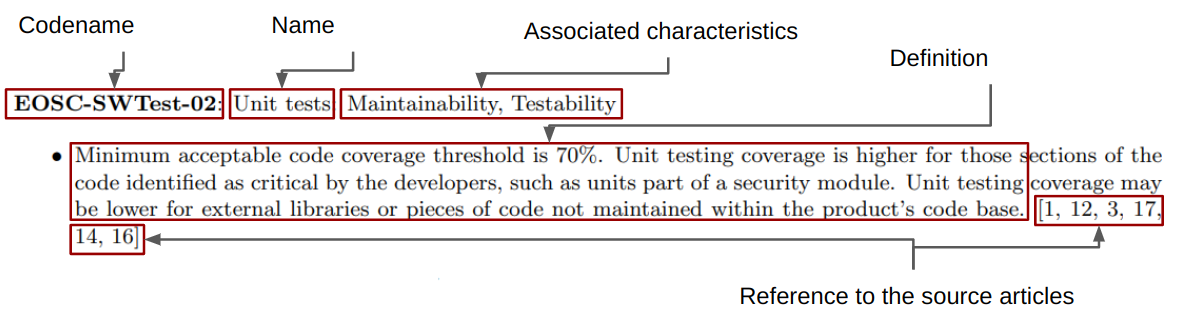
\includegraphics[width=0.99\linewidth]{imgs/qa.png}
    \caption{The structure of each Attribute or Metric entry, as it appears in the Appendix.}
    \label{fig:sqattr}
\end{figure}
